%%%%%%%%%%%%%%%%%%%%%%%%%%%%%%%%%%%%%%%%%%%%%%%%%%%%%%%%%%%%%%%%%%%%%%%%%%%%%%%%
\section{Considerações iniciais}

Sistemas de reconhecimento de imagens comumente utilizam uma imagem em níveis de cinza (8-bits -- 256 intensidades) para as etapas subsequentes à extração de características. Ao aplicar a quantização (redução de cores) na etapa de pré-processamento, é esperada a redução da complexidade do vetor de características logo no início, beneficiando todos os passos subsequentes.

Para analisar o impacto do uso da quantização, diferentes parâmetros de quantização combinados com quatro métodos de extração de cor e um de textura são utilizados. Esses métodos foram escolhidos de acordo com os resultados apresentados por \citeonline{Penatti2012}, com exceção de HOG e LBP, que também são descritores frequentemente utilizados na literatura \cite{Wang2009a}.

Este capítulo descorre sobre a quantização das imagens antes da extração de características. Os métodos utilizados foram apresentados na Seção~\ref{sec:quantizacao}.

%%%%%%%%%%%%%%%%%%%%%%%%%%%%%%%%%%%%%%%%%%%%%%%%%%%%%%%%%%%%%%%%%%%%%%%%%%%%%%%%
\section{Quantização de imagens}

O pipeline de reconhecimento de imagens envolve um passo de converter imagens coloridas em imagens com apenas um canal, obtendo uma imagem quantizada que pode ser então processada por métodos de extração de características. Dessa forma, cada imagem -- originalmente no espaço de cor RGB -- é convertida a um único canal com $C$ níveis de intensidade. Após, são utilizados os métodos apresentados na Seção \ref{sec:extracao} para extrair as características.
A Figura \ref{fig:quant:quantizationFlow} ilustra esses passos, da aquisição até a classificação das imagens.

\begin{figure}[!htbp]
  \begin{center}
    \centering
    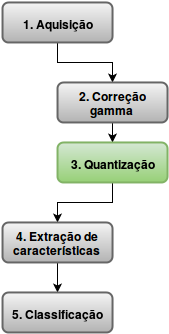
\includegraphics[width=0.25\linewidth]{\detokenize{figuras/quantizacao/quantizationFlow.png}}
  \end{center}
  \caption[O pipeline de reconhecimento de imagens pode envolver uma etapa de converter imagens coloridas em imagens em escala de cinza, obtendo uma imagem quantizada que pode ser então processada por métodos de extração de características. O vetor com essas características é então dado como entrada a algum método de classificação.]{O pipeline de reconhecimento de imagens pode envolver uma etapa de converter imagens coloridas em imagens em escala de cinza, obtendo uma imagem quantizada que pode ser então processada por métodos de extração de características. O vetor com essas características é então dado como entrada a algum método de classificação. \textit{Fonte:~Elaborado pela autora.}}
  \label{fig:quant:quantizationFlow}
\end{figure}

Cada método de quantização se comporta diferentemente para uma dada imagem RGB. Por exemplo, o método \emph{Intensidade} mapeia todas as permutações dos mesmos valores em RBG para a mesma cor. Dessa forma, produz um plano no cubo RBG conforme mostrado na Figura \ref{fig:quant:plano}. O efeito do \emph{Gleam} é similar, mas dada a natureza da função \textit{gamma}, cobrindo uma superfície curva. Em todos os casos, o resultado é o mapeamento de características cromáticas bem diferentes em valores de intensidades similares. Os métodos Luminância e Luma tentam melhorar um pouco isso ao ponderar a combinação linear dos canais.

\begin{figure}[!htbp]
  \begin{center}
    \centering
    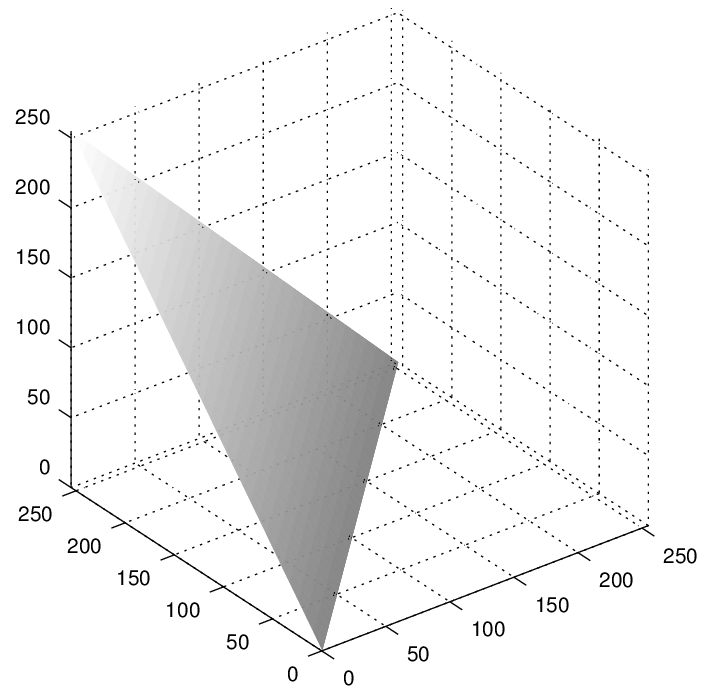
\includegraphics[width=0.5\linewidth]{\detokenize{figuras/quantizacao/plano.png}}
  \end{center}
  \caption[Plano computado pelo método de conversão para escala de cinza \emph{Intensidade}, quando um dos canais de cor possui valor 255.]{Plano computado pelo método de conversão para escala de cinza \emph{Intensidade}, quando um dos canais de cor possui valor 255. \textit{Fonte:~\cite{Ponti2016}.}}
  \label{fig:quant:plano}
\end{figure}

Um exemplo das imagens obtidas após os métodos de quantização apresentados anteriormente pode ser visto na Figura \ref{fig:quant:quantizacoes}. A barra de gradientes abaixo da imagem dos pincéis demonstra como os métodos de quantização se comportam dada a variação da cor. É possível notar que os métodos \emph{Luminância} e \emph{MSB} conseguiram melhor discriminar as cores. Além disso, o mapa de cores \emph{MSB} obteve um maior número de cores únicas.

\begin{figure}[!htbp]
  \begin{center}
    \begin{subfigure}{.25\textwidth}
      \centering
      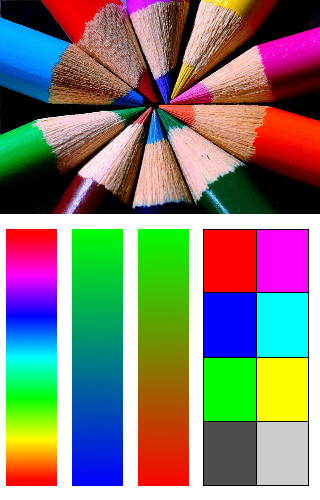
\includegraphics[width=\linewidth]{\detokenize{figuras/quantizacao/fig_quanttest.png}}
      \caption{Original}
      \label{fig:quant:original}
    \end{subfigure}
    \begin{subfigure}{.25\textwidth}
      \centering
      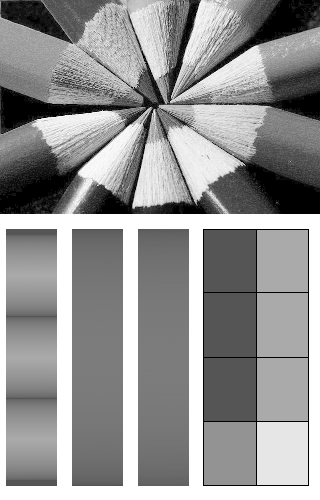
\includegraphics[width=\linewidth]{\detokenize{figuras/quantizacao/fig_quantGleam.png}}
      \caption{Gleam}
    \end{subfigure}
    \begin{subfigure}{.25\textwidth}
      \centering
      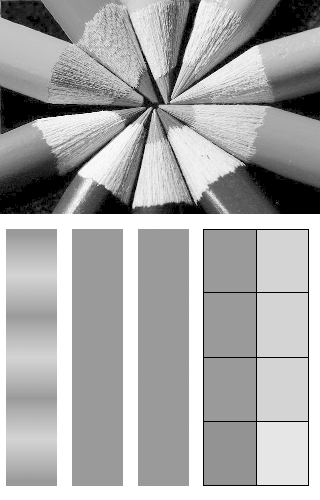
\includegraphics[width=\linewidth]{\detokenize{figuras/quantizacao/fig_quantIntensity.png}}
      \caption{Intensidade'}
    \end{subfigure}
    \begin{subfigure}{.25\textwidth}
      \centering
      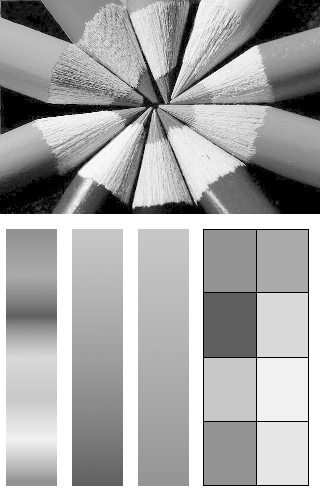
\includegraphics[width=\linewidth]{\detokenize{figuras/quantizacao/fig_quantLuminance.png}}
      \caption{Luminance'}
    \end{subfigure}
    \begin{subfigure}{.25\textwidth}
      \centering
      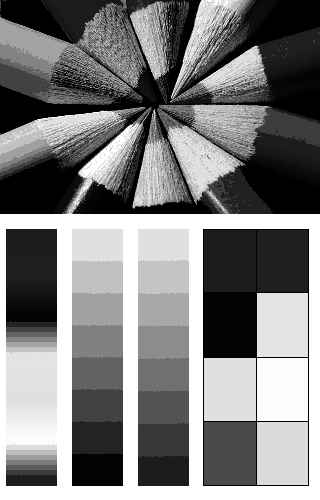
\includegraphics[width=\linewidth]{\detokenize{figuras/quantizacao/fig_quantMSB.png}}
      \caption{MSB}
    \end{subfigure}
    \hspace{0.1\textwidth}
  \end{center}
  \caption[Resultado da aplicação de métodos de quantização. A imagem original \protect\subref{fig:quant:original} resultou em versões de um canal de cor com 232 cores unicas para MSB e 184 cores para os restantes métodos.]{Resultado da aplicação de métodos de quantização. A imagem original \protect\subref{fig:quant:original} resultou em versões de um canal de cor com 232 cores unicas para MSB e 184 cores para os restantes métodos. \textit{Fonte:~\cite{Ponti2016}.}}
  \label{fig:quant:quantizacoes}
\end{figure}

% A Tabela \ref{tab:quantizacao} apresenta alguns exemplos numéricos, com a saída de cada método. Nesse caso, as entradas são tuplas de valores $(R, G, B)$. Note que a correção \textit{gamma} deve ser computada em um intervalo de valores reais $0-1$, que depois é mapeado para o intervalo $0-255$.

A Figura \ref{fig:quant:avioes} apresenta um exemplo de redução de cores utilizando o método \emph{MSB} para um par de imagens da base de dados \emph{Caltech-101}. É possível notar que há uma certa preservação das cores, especialmente entre a utilização de 64 e 256 níveis. Com apenas 32 cores as imagens ainda lembram a sua versão original, mas há uma perda considerável de informação.

\begin{figure}[!htbp]
  \begin{center}
    \centering
    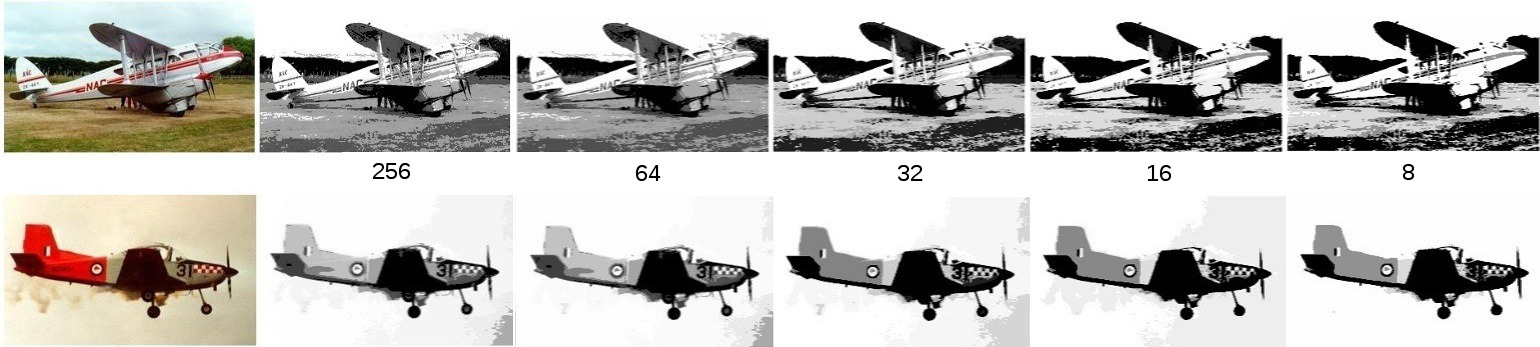
\includegraphics[width=\linewidth]{\detokenize{figuras/quantizacao/fig_quantizationexample.jpg}}
  \end{center}
  \caption[Duas imagens da base de dados \emph{Caltech101} com variações no parâmetro de cor utilizando o método \emph{MSB}. Da esquerda para a direita: imagem original 24-bits e suas versões quantizadas com: 256, 64, 32, 16 e 8 cores.]{Duas imagens da base de dados \emph{Caltech101} com variações no parâmetro de cor utilizando o método \emph{MSB}. Da esquerda para a direita: imagem original 24-bits e suas versões quantizadas com: 256, 64, 32, 16 e 8 cores. \textit{Fonte:~\cite{Ponti2016}.}}
  \label{fig:quant:avioes}
\end{figure}

%%%%%%%%%%%%%%%%%%%%%%%%%%%%%%%%%%%%%%%%%%%%%%%%%%%%%%%%%%%%%%%%%%%%%%%%%%%%%%%%
\section{Considerações finais}

Os resultados da utilização dos métodos descritos neste capítulo estão no Capítulo \ref{cap:resultados}.
